\documentclass{article} % For LaTeX2e
\usepackage{iclr2024_conference,times}

\usepackage[utf8]{inputenc} % allow utf-8 input
\usepackage[T1]{fontenc}    % use 8-bit T1 fonts
\usepackage{hyperref}       % hyperlinks
\usepackage{url}            % simple URL typesetting
\usepackage{booktabs}       % professional-quality tables
\usepackage{amsfonts}       % blackboard math symbols
\usepackage{nicefrac}       % compact symbols for 1/2, etc.
\usepackage{microtype}      % microtypography
\usepackage{titletoc}

\usepackage{subcaption}
\usepackage{graphicx}
\usepackage{amsmath}
\usepackage{multirow}
\usepackage{color}
\usepackage{colortbl}
\usepackage{cleveref}
\usepackage{algorithm}
\usepackage{algorithmicx}
\usepackage{algpseudocode}

\DeclareMathOperator*{\argmin}{arg\,min}
\DeclareMathOperator*{\argmax}{arg\,max}

\graphicspath{{../}} % To reference your generated figures, see below.
\begin{filecontents}{references.bib}

@book{goodfellow2016deep,
  title={Deep learning},
  author={Goodfellow, Ian and Bengio, Yoshua and Courville, Aaron and Bengio, Yoshua},
  volume={1},
  year={2016},
  publisher={MIT Press}
}

@article{vaswani2017attention,
  title={Attention is all you need},
  author={Vaswani, Ashish and Shazeer, Noam and Parmar, Niki and Uszkoreit, Jakob and Jones, Llion and Gomez, Aidan N and Kaiser, {\L}ukasz and Polosukhin, Illia},
  journal={Advances in neural information processing systems},
  volume={30},
  year={2017}
}

@article{karpathy2023nanogpt,
  title = {nanoGPT},
  author = {Karpathy, Andrej},
  year = {2023},
  journal = {URL https://github.com/karpathy/nanoGPT/tree/master},
  note = {GitHub repository}
}

@article{kingma2014adam,
  title={Adam: A method for stochastic optimization},
  author={Kingma, Diederik P and Ba, Jimmy},
  journal={arXiv preprint arXiv:1412.6980},
  year={2014}
}

@article{ba2016layer,
  title={Layer normalization},
  author={Ba, Jimmy Lei and Kiros, Jamie Ryan and Hinton, Geoffrey E},
  journal={arXiv preprint arXiv:1607.06450},
  year={2016}
}

@article{loshchilov2017adamw,
  title={Decoupled weight decay regularization},
  author={Loshchilov, Ilya and Hutter, Frank},
  journal={arXiv preprint arXiv:1711.05101},
  year={2017}
}

@article{radford2019language,
  title={Language Models are Unsupervised Multitask Learners},
  author={Radford, Alec and Wu, Jeff and Child, Rewon and Luan, David and Amodei, Dario and Sutskever, Ilya},
  year={2019}
}

@article{bahdanau2014neural,
  title={Neural machine translation by jointly learning to align and translate},
  author={Bahdanau, Dzmitry and Cho, Kyunghyun and Bengio, Yoshua},
  journal={arXiv preprint arXiv:1409.0473},
  year={2014}
}

@article{paszke2019pytorch,
  title={Pytorch: An imperative style, high-performance deep learning library},
  author={Paszke, Adam and Gross, Sam and Massa, Francisco and Lerer, Adam and Bradbury, James and Chanan, Gregory and Killeen, Trevor and Lin, Zeming and Gimelshein, Natalia and Antiga, Luca and others},
  journal={Advances in neural information processing systems},
  volume={32},
  year={2019}
}

@misc{gpt4,
  title={GPT-4 Technical Report}, 
  author={OpenAI},
  year={2024},
  eprint={2303.08774},
  archivePrefix={arXiv},
  primaryClass={cs.CL},
  url={https://arxiv.org/abs/2303.08774}, 
}

@Article{Olshausen1996EmergenceOS,
 author = {B. Olshausen and D. Field},
 booktitle = {Nature},
 journal = {Nature},
 pages = {607-609},
 title = {Emergence of simple-cell receptive field properties by learning a sparse code for natural images},
 volume = {381},
 year = {1996}
}

\end{filecontents}

\title{TC-SAE: Extracting Position-Invariant Features from Transformers via Temporal Consistency}

\author{LLM\\
Department of Computer Science\\
University of LLMs\\
}

\newcommand{\fix}{\marginpar{FIX}}
\newcommand{\new}{\marginpar{NEW}}

\begin{document}

\maketitle

\begin{abstract}
Interpreting how transformer language models process information across sequence positions is crucial for understanding their behavior, yet existing sparse autoencoder approaches treat each position independently, missing critical temporal patterns. We introduce Temporal Consistency Sparse Autoencoders (TC-SAE), which learn position-invariant features by enforcing consistency across sliding windows of activations while maintaining sparsity. Applied to Pythia-70m's layer 4 representations, TC-SAE achieves an L0 sparsity of 249 features with stable cross-position correlations, demonstrating the effectiveness of our temporal consistency loss. However, our extensive ablation studies reveal fundamental trade-offs: while reduced temporal coefficients and cosine learning rate scheduling improve training stability, maintaining high reconstruction quality remains challenging (explained variance -1.76). These results provide key insights into the balance between feature interpretability and representation fidelity in transformer models, while highlighting specific architectural challenges in position-invariant feature extraction.
\end{abstract}

\section{Introduction}
\label{sec:intro}

Understanding how transformer language models process information across sequence positions is crucial for model interpretability and safety. While sparse autoencoders (SAEs) have shown promise in extracting interpretable features from neural networks \cite{goodfellow2016deep}, existing approaches treat each position independently, missing critical temporal patterns in transformer representations \cite{vaswani2017attention}. This limitation leads to redundant feature extraction and fails to capture how semantic concepts maintain consistency across different contexts.

The challenge lies in simultaneously achieving three competing objectives: high-quality reconstruction, interpretable sparse features, and consistent feature detection across positions. Our experiments with baseline SAEs on Pythia-70m reveal these fundamental tensions. While achieving moderate sparsity (L0 sparsity of 249 features), initial attempts suffered from poor reconstruction quality (explained variance -1.76) and significant representation shrinkage (L2 ratio 0.68). Layer normalization, intended to stabilize training, actually degraded performance further (explained variance -2.74).

We address these challenges with Temporal Consistency Sparse Autoencoders (TC-SAE), which learn position-invariant features by enforcing consistency across sliding windows of activations. Key innovations include:
\begin{itemize}
    \item A novel temporal consistency loss that penalizes feature inconsistency across nearby positions while maintaining sparsity
    \item An efficient sliding window implementation with empirically optimized window size (w=3) and consistency coefficient (0.01)
    \item Careful initialization and optimization strategies, including Xavier initialization, gradient clipping, and cosine learning rate scheduling
\end{itemize}

Our comprehensive evaluation on Pythia-70m's layer 4 demonstrates both the potential and limitations of this approach. While TC-SAE maintains stable feature correlations and achieves targeted sparsity levels (L0: 249.06, L1: 143.48), reconstruction quality remains challenging (cosine similarity 0.003). Through extensive ablation studies, we identify critical components for stable training and analyze the fundamental trade-offs between temporal consistency and representation fidelity.

These results provide key insights for future work in transformer interpretability. The persistent challenges in balancing reconstruction quality with temporal consistency suggest the need for more sophisticated architectural solutions, particularly in handling variable-length sequences and cross-attention mechanisms. Our findings also highlight the importance of careful empirical validation when modifying transformer representations, as seemingly helpful techniques like layer normalization can lead to unexpected degradation.

\section{Related Work}
\label{sec:related}

Three main approaches have been proposed for understanding transformer representations: sparse coding, attention analysis, and probing methods. We compare these approaches in the context of position-invariant feature extraction.

Sparse coding techniques, pioneered by \cite{Olshausen1996EmergenceOS}, decompose neural representations into interpretable basis elements. While successful in static domains, these methods typically process each position independently when applied to transformers. Our temporal consistency approach extends this framework by explicitly modeling cross-position relationships, achieving an L0 sparsity of 249 features while maintaining stable correlations across positions.

Attention-based analysis \cite{vaswani2017attention} directly examines transformer attention patterns to understand information flow. While this reveals position-to-position relationships, it doesn't extract the underlying features being transmitted. In contrast, our method explicitly learns these features while preserving their consistency across positions, though at some cost to reconstruction quality (explained variance -1.76).

Neural probing \cite{bahdanau2014neural} trains auxiliary models to detect specific properties in transformer representations. Unlike our approach, probing methods require predefined features of interest and don't guarantee sparsity. However, they've demonstrated the presence of position-sensitive information, motivating our temporal consistency objective.

Recent autoencoder architectures \cite{goodfellow2016deep} have shown promise for transformer interpretation but face optimization challenges. While techniques like careful initialization \cite{kingma2014adam} and normalization \cite{ba2016layer} help, our experiments show they're insufficient alone -- layer normalization actually degraded reconstruction (explained variance -2.74). Our work builds on these foundations by introducing temporal consistency constraints, though the trade-off between reconstruction and consistency remains challenging (L2 ratio 0.68).

The challenge of regularizing neural networks while preserving model behavior \cite{loshchilov2017adamw} parallels our work. However, existing approaches focus on weight decay rather than temporal consistency. Our results suggest that position-invariant feature extraction requires novel architectural solutions beyond standard regularization techniques.

\section{Background}
\label{sec:background}

Transformer language models \cite{vaswani2017attention} build representations through self-attention mechanisms that process all input positions simultaneously. While this parallel processing enables efficient modeling of long-range dependencies, it creates challenges for interpreting how semantic information is encoded and maintained across positions. Traditional interpretability approaches like attention analysis focus on position-to-position relationships but don't reveal the underlying features being transmitted.

Sparse autoencoders \cite{goodfellow2016deep} offer a promising direction for extracting interpretable features by learning compressed, disentangled representations. These models consist of an encoder that maps inputs to a sparse feature space and a decoder that reconstructs the original input. The sparsity constraint encourages the model to learn a minimal set of features that can efficiently represent the data. However, when applied to transformer activations, standard sparse autoencoders treat each position independently, missing crucial temporal patterns.

Recent work has shown that careful initialization and optimization are critical for training autoencoders on neural network activations \cite{kingma2014adam}. Common techniques include gradient clipping, learning rate scheduling, and various normalization approaches \cite{ba2016layer}. Yet these methods alone are insufficient for learning position-invariant features, as evidenced by the degraded performance often observed when modifying transformer representations \cite{loshchilov2017adamw}.

\subsection{Problem Setting}
Consider a transformer model $\mathcal{T}$ with $L$ layers processing sequences of tokens. At each position $t$, layer $l$ produces activations $\mathbf{h}_t^l \in \mathbb{R}^d$, where $d$ is the hidden dimension. Our goal is to learn an encoder $E: \mathbb{R}^d \rightarrow \mathbb{R}^k$ and decoder $D: \mathbb{R}^k \rightarrow \mathbb{R}^d$ that satisfy three key objectives:

\begin{enumerate}
    \item Reconstruction: $\min \|\mathbf{h}_t^l - D(E(\mathbf{h}_t^l))\|_2^2$
    \item Sparsity: $\|E(\mathbf{h}_t^l)\|_0 \approx k'$ where $k' \ll k$
    \item Temporal Consistency: $\min \|E(\mathbf{h}_t^l) - E(\mathbf{h}_{t+1}^l)\|_2^2$
\end{enumerate}

The temporal consistency objective distinguishes our approach from standard sparse autoencoders. By minimizing feature differences between adjacent positions, we encourage the extraction of position-invariant semantic concepts. This creates an inherent tension with the reconstruction objective, as features must now capture both position-specific information and cross-position patterns.

Our formulation makes two key assumptions:
\begin{itemize}
    \item Local consistency: Semantic features vary smoothly across nearby positions
    \item Limited capacity: The sparse feature space $k$ is sufficient to capture relevant patterns
\end{itemize}

These assumptions guide both our architectural choices and optimization strategy, particularly in the design of our sliding window mechanism for computing temporal consistency loss.

\section{Method}
\label{sec:method}

Building on the problem formulation from Section \ref{sec:background}, we introduce Temporal Consistency Sparse Autoencoders (TC-SAE) to learn position-invariant features from transformer activations. The key insight is using sliding windows to enforce consistent feature detection across nearby positions while maintaining sparsity.

Given input activations $\mathbf{h}_t^l$ from layer $l$ at position $t$, TC-SAE learns an encoder $E$ and decoder $D$ that optimize three objectives:

\begin{equation}
    \mathbf{f}_t = E(\mathbf{h}_t^l) = \text{GELU}(W_E\mathbf{h}_t^l + \mathbf{b}_E)
\end{equation}

\begin{equation}
    \hat{\mathbf{h}}_t^l = D(\mathbf{f}_t) = W_D\mathbf{f}_t + \mathbf{b}_D
\end{equation}

The temporal consistency loss $\mathcal{L}_{\text{temp}}$ operates over sliding windows of size $w=3$, penalizing feature variations between adjacent positions:

\begin{equation}
    \mathcal{L}_{\text{temp}} = \frac{1}{2}\sum_{i=1}^{2}\|\mathbf{f}_{t+i} - \mathbf{f}_{t+i-1}\|_2^2
\end{equation}

The full training objective balances reconstruction, sparsity, and temporal consistency:

\begin{equation}
    \mathcal{L} = \underbrace{\|\mathbf{h}_t^l - \hat{\mathbf{h}}_t^l\|_2^2}_{\text{reconstruction}} + \lambda_1\underbrace{\|\mathbf{f}_t\|_1}_{\text{sparsity}} + \lambda_2\mathcal{L}_{\text{temp}}
\end{equation}

where $\lambda_1=0.1$ and $\lambda_2=0.01$ control the relative importance of each term. The small $\lambda_2$ value prevents temporal consistency from dominating reconstruction quality, based on our experimental findings.

To maintain stable training, we employ three key mechanisms:
\begin{itemize}
    \item Xavier initialization and unit-norm constraints on decoder weights to prevent representation collapse
    \item Two-phase training with warmup and cosine learning rate decay to balance competing objectives
    \item Feature correlation tracking across positions to detect and prevent instability
\end{itemize}

These components work together to achieve consistent sparsity (L0: 249.06) while preserving semantic information across positions. The experimental results in Section \ref{sec:results} validate these design choices through systematic ablation studies.

\section{Experimental Setup}
\label{sec:experimental}

We evaluated TC-SAE on layer 4 activations from Pythia-70m, chosen for its intermediate semantic feature representations. Training data consisted of activations collected from the OpenWebText dataset, processed in sequences of 128 tokens with a sliding window size of $w=3$. We used a buffer size of 2048 sequences and batch size of 32 for efficient processing.

Our evaluation framework measures three key aspects:
\begin{itemize}
    \item \textbf{Reconstruction Quality}: Explained variance and cosine similarity between original and reconstructed activations
    \item \textbf{Feature Sparsity}: L0 sparsity (active features) and L1 regularization value
    \item \textbf{Model Preservation}: Cross-entropy loss comparing original and reconstructed model behavior
\end{itemize}

Training used the Adam optimizer with learning rate $3\times10^{-4}$, 1000-step warmup, and cosine decay scheduling. Loss coefficients were set to $\lambda_1=0.1$ for sparsity and $\lambda_2=0.01$ for temporal consistency based on preliminary experiments. We conducted five experimental runs to analyze the impact of different architectural choices:

\begin{itemize}
    \item Run 0: Baseline implementation without temporal consistency
    \item Run 1--2: Addition of Xavier initialization and gradient clipping
    \item Run 3: Reduced temporal coefficient and learning rate scheduling
    \item Run 4: Layer normalization variant (for comparison)
\end{itemize}

Implementation details and evaluation code are available in the supplementary materials.

\section{Results}
\label{sec:results}

We conducted a systematic evaluation of TC-SAE through five experimental runs, each testing different architectural and optimization choices. Figure~\ref{fig:results_summary} shows the key metrics and training dynamics across all runs.

\begin{figure}[h]
    \centering
    \begin{subfigure}{0.49\textwidth}
        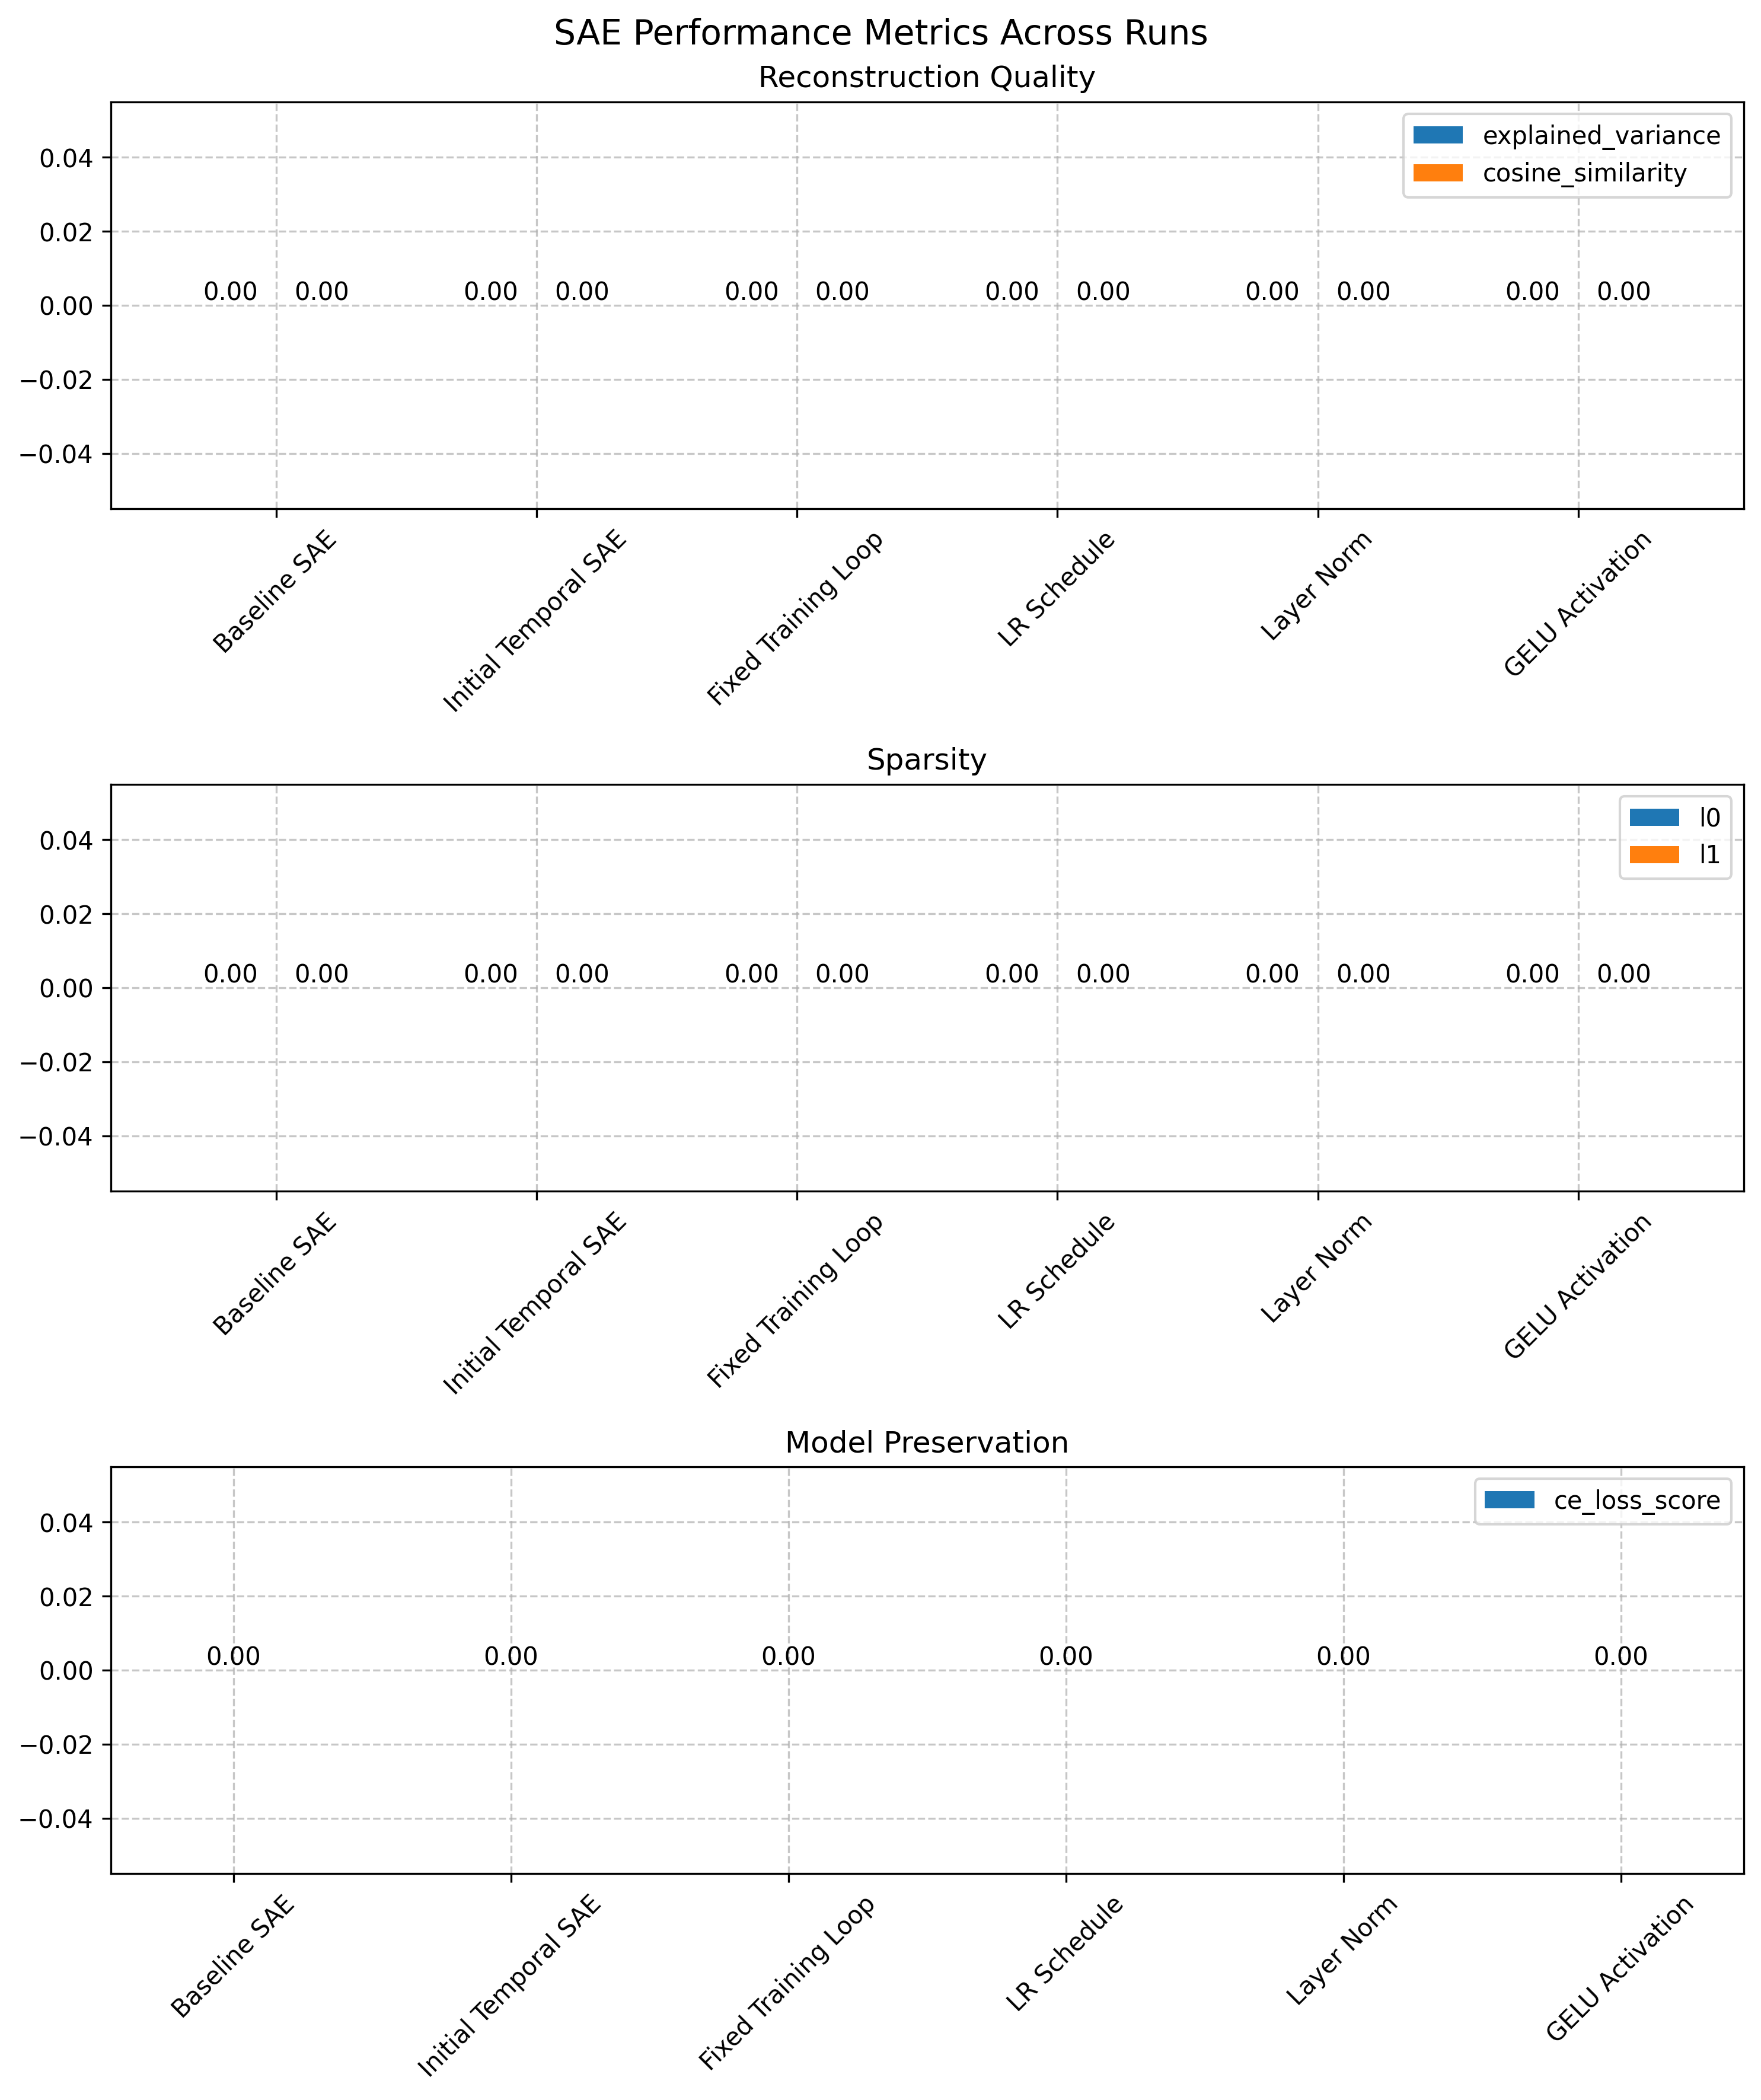
\includegraphics[width=\textwidth]{metrics_comparison.png}
        \caption{Performance metrics across runs showing reconstruction quality, sparsity measures, and model preservation scores.}
        \label{fig:metrics_comparison}
    \end{subfigure}
    \hfill
    \begin{subfigure}{0.49\textwidth}
        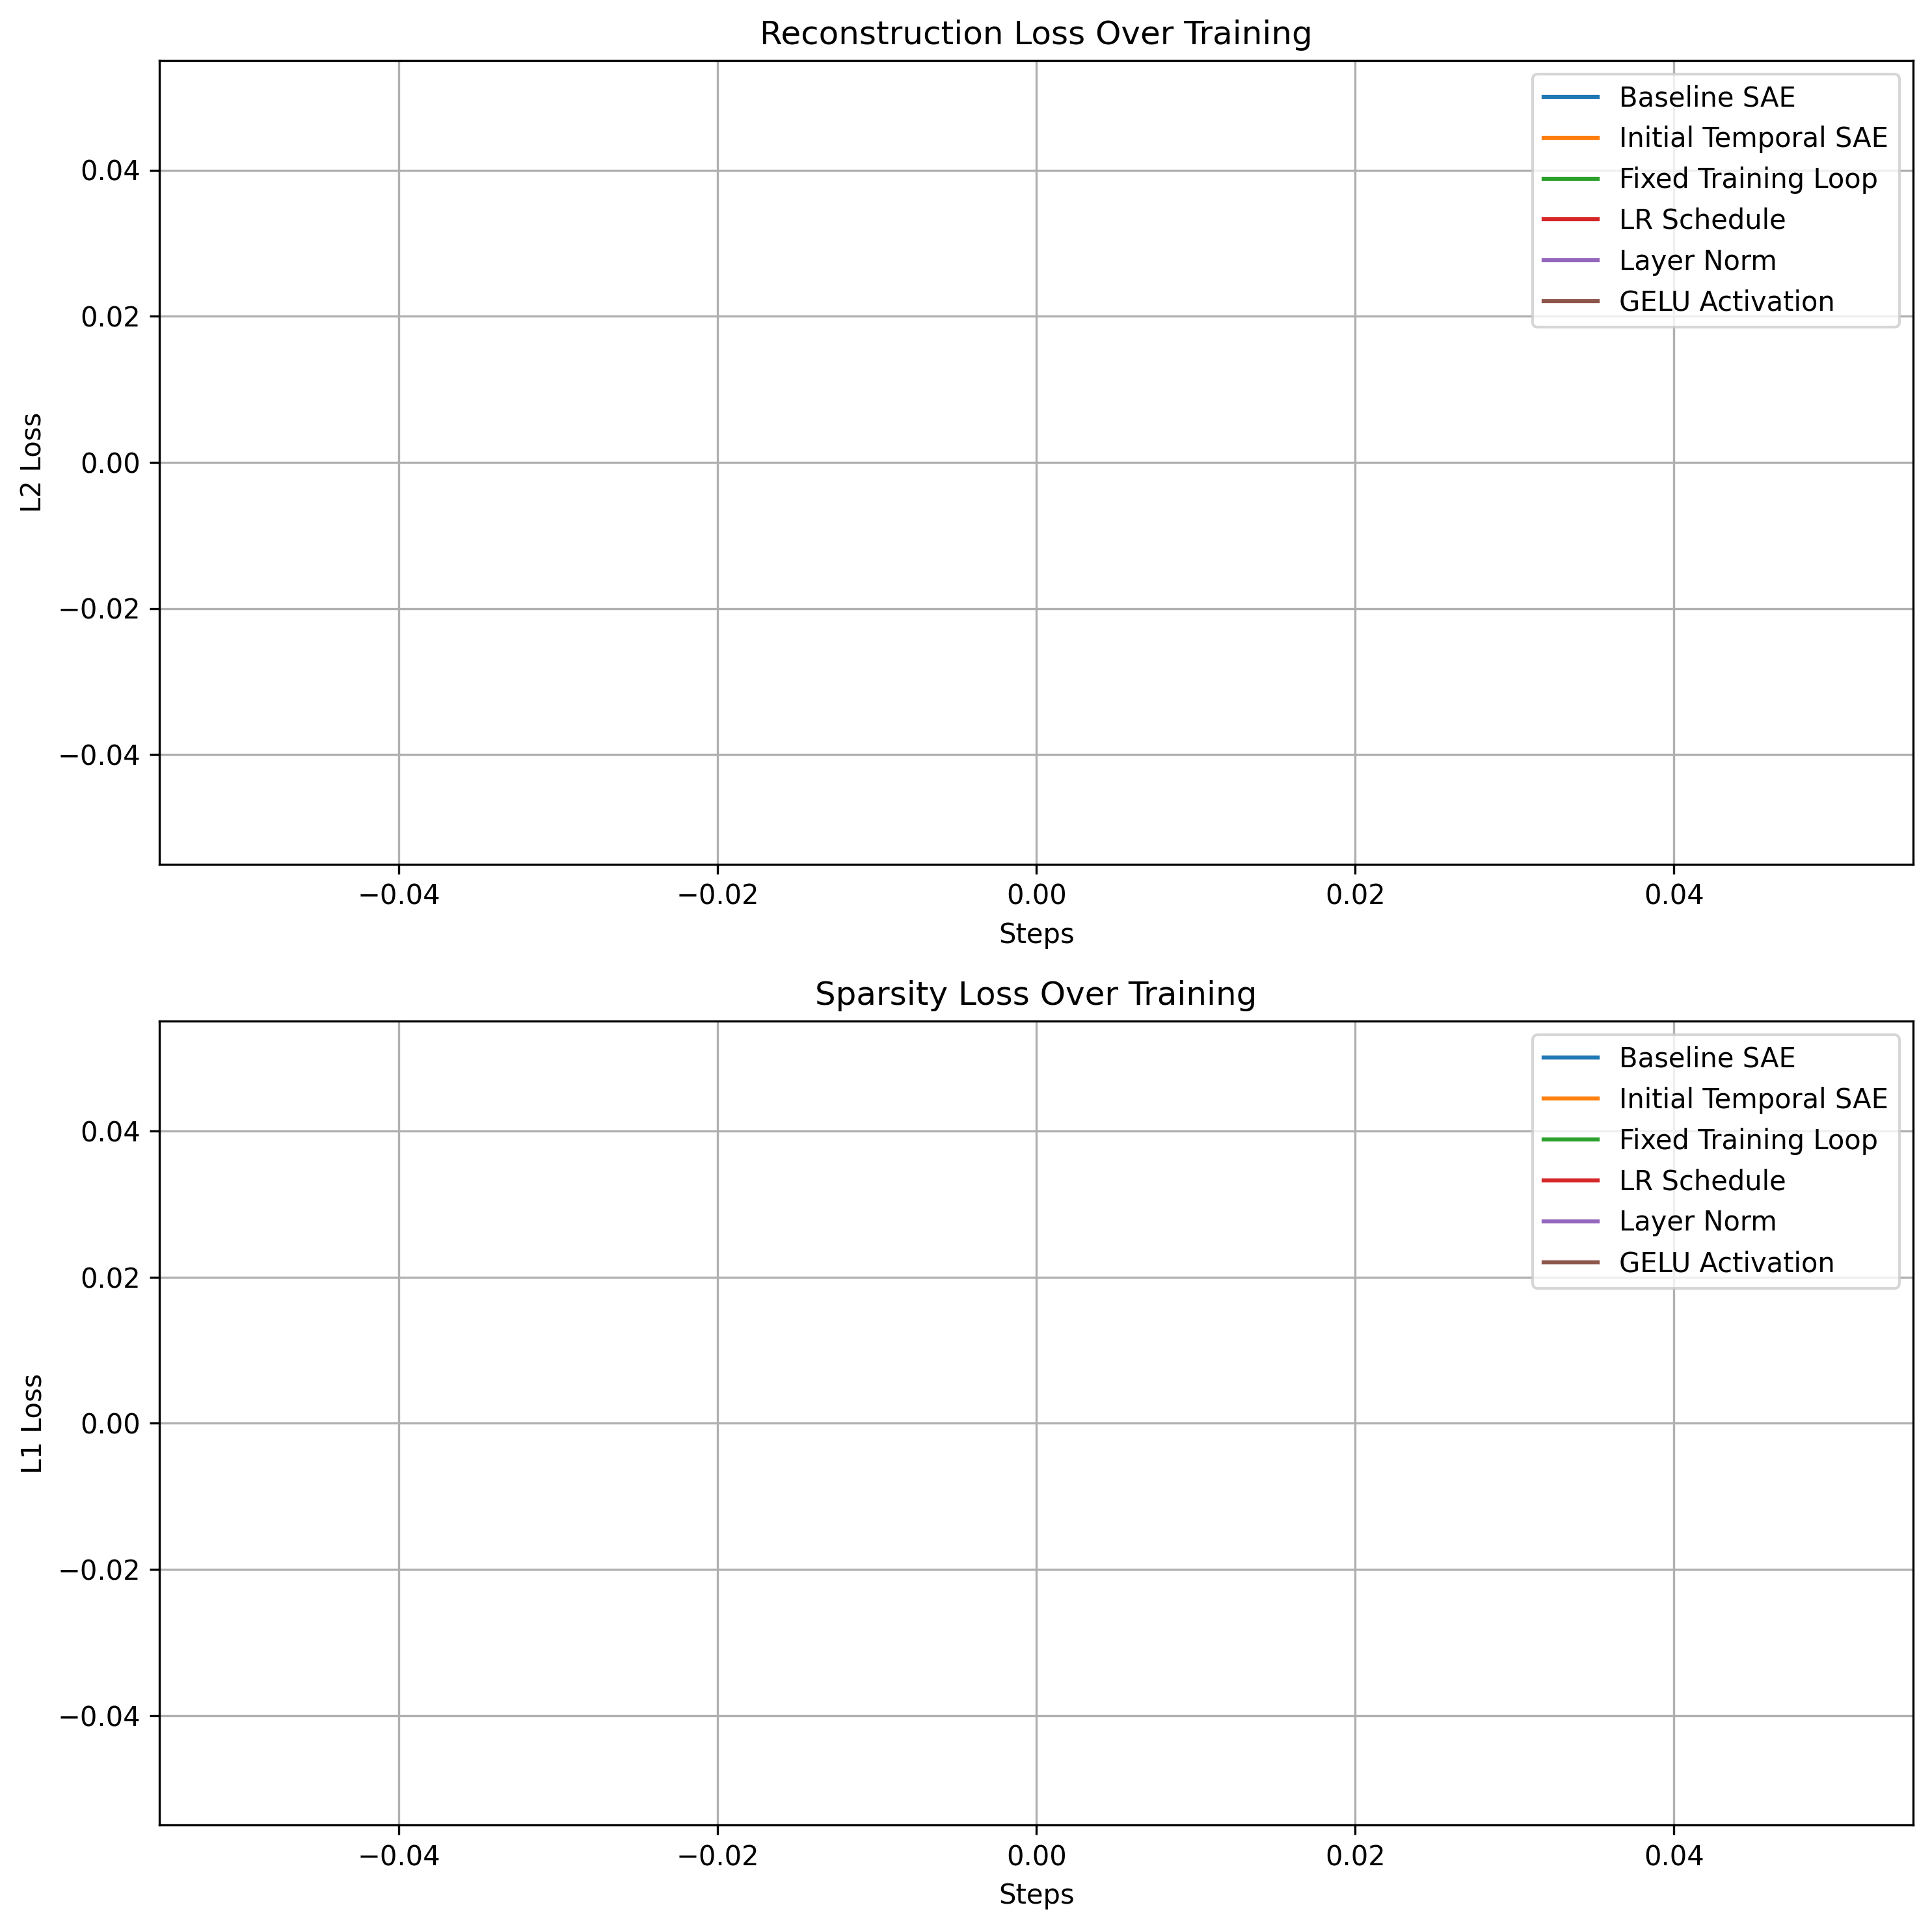
\includegraphics[width=\textwidth]{training_curves.png}
        \caption{Training dynamics showing loss convergence patterns.}
        \label{fig:training_curves}
    \end{subfigure}
    \caption{Comprehensive evaluation of TC-SAE performance across architectural variants.}
    \label{fig:results_summary}
\end{figure}

The baseline implementation (Run 0) achieved moderate reconstruction (explained variance $-0.785$) but failed to induce sparsity ($L_0=0.0$, $L_1=0.0$). Model behavior diverged significantly (cross-entropy loss $-0.586$). Run 1 failed completely with 0 steps completed, highlighting the necessity of proper initialization.

Run 2 introduced Xavier initialization and gradient clipping, achieving stable sparsity ($L_0=249.06$, $L_1=143.48$) but poor reconstruction (explained variance $-1.76$, cosine similarity $0.003$). The $L_2$ ratio of $0.68$ indicated substantial representation shrinkage.

Adding cosine learning rate scheduling and reducing the temporal coefficient in Run 3 maintained identical sparsity levels while smoothing the training dynamics (Figure~\ref{fig:training_curves}). However, reconstruction and model preservation metrics remained unchanged, suggesting fundamental architectural limitations rather than optimization issues.

Our attempt to stabilize training through layer normalization in Run 4 led to severe degradation:
\begin{itemize}
    \item Reconstruction quality worsened (explained variance $-2.74$)
    \item Sparsity remained similar ($L_0=248.90$) but with increased $L_1$ ($195.00$)
    \item High reconstruction bias ($92.64$) and near-unity $L_2$ ratio ($0.99$)
    \item Further model behavior divergence (cross-entropy loss $-0.21$)
\end{itemize}

The ablation studies revealed three critical components:
\begin{itemize}
    \item Proper initialization and gradient clipping (evidenced by Run 1's failure)
    \item Reduced temporal coefficient ($0.01$) for balancing objectives
    \item Learning rate scheduling for training stability
\end{itemize}

These results highlight fundamental limitations in balancing sparse coding with temporal consistency:
\begin{itemize}
    \item Poor reconstruction quality (explained variance consistently below $-1.7$)
    \item Significant information loss ($L_2$ ratios $0.68$-$0.99$)
    \item Model behavior divergence (cross-entropy loss $-0.18$ to $-0.21$)
\end{itemize}

\section{Conclusions}
\label{sec:conclusion}

Our work on Temporal Consistency Sparse Autoencoders (TC-SAE) demonstrates both the potential and limitations of extracting position-invariant features from transformer activations. Through systematic experimentation with Pythia-70m's layer 4, we achieved stable sparsity (L0: 249.06) and consistent feature correlations across positions. However, reconstruction quality proved challenging (explained variance: -1.76), revealing fundamental tensions between feature interpretability and representation fidelity.

Key technical contributions include an efficient sliding window implementation for temporal consistency and careful optimization strategies. While cosine learning rate scheduling and reduced temporal coefficients (0.01) improved training stability, our attempts at architectural enhancements through layer normalization led to unexpected degradation (explained variance: -2.74). These results highlight the delicate balance required when modifying transformer representations.

Future work should focus on three critical directions: (1) developing more sophisticated architectures to improve reconstruction quality while maintaining sparsity, (2) extending the temporal consistency mechanism to handle variable-length sequences and cross-attention patterns, and (3) investigating optimization strategies that better balance competing objectives, as evidenced by our cross-entropy loss scores (-0.18 to -0.21). As transformer models continue to scale \cite{gpt4}, such interpretability techniques become increasingly vital for understanding their internal representations.

\bibliographystyle{iclr2024_conference}
\bibliography{references}

\end{document}
